\documentclass[10pt,a4paper]{article}
\usepackage[T1]{fontenc}
\usepackage[utf8]{inputenc}
\usepackage[spanish,es-tabla]{babel}
\parindent=0cm %Modificar tamaño de sangria
\usepackage{amsmath}
\usepackage{amssymb,amsfonts,latexsym,cancel}
\usepackage{graphicx}
\usepackage{epstopdf}
\usepackage{float}
\usepackage{subfigure}
\usepackage{array}
\usepackage{longtable}
\newcolumntype{E}{>{$}c<{$}}
\setcounter{MaxMatrixCols}{40}
\usepackage{bm}
\usepackage{xcolor}
%%%%%%%%%%%%%%%%%%%%%%%%%%%%%%%%%%%%%
%%%PAQUETES O CONFIGURACION NUEVA%%%%
%%%%%%%%%%%%%%%%%%%%%%%%%%%%%%%%%%%%%
\usepackage[lmargin=2cm, rmargin=2cm,top=2.5cm,bottom=2cm]{geometry}
\usepackage{fancyhdr}
\pagestyle{fancy}
\fancyhead{}%%Es para limpiar el documento
\fancyhead[C]{Calculo Vectorial Integral }
\fancyhead[R]{
\includegraphics[scale=0.07]{figuras/logo}}
\fancyfoot{}
\fancyfoot[R]{\thepage}
\fancyfoot[L]{Bryan Ricardo}
\renewcommand{\headrulewidth}{0.9pt}
\renewcommand{\footrulewidth}{0.5pt}
\usepackage{xcolor}
\providecommand{\abs}[1]{\lvert#1\rvert}
\providecommand{\norm}[1]{\lVert#1\rVert}
\usepackage{ mathrsfs }
%%%%%%%%%%%%%%%%%%%%%%%%%%%%%%%%%%%%%
%%INTEGRALES INFERIORES Y SUPERIORES
\usepackage{amsmath}
\def\upint{\mathchoice%
    {\mkern13mu\overline{\vphantom{\intop}\mkern7mu}\mkern-20mu}%
    {\mkern7mu\overline{\vphantom{\intop}\mkern7mu}\mkern-14mu}%
    {\mkern7mu\overline{\vphantom{\intop}\mkern7mu}\mkern-14mu}%
    {\mkern7mu\overline{\vphantom{\intop}\mkern7mu}\mkern-14mu}%
  \int}
\def\lowint{\mkern3mu\underline{\vphantom{\intop}\mkern7mu}\mkern-10mu\int}
%%%%%%%%%%%%%%%%%%%%%%%%%%%%%%%%%%%%%%%%%%%%%%%
\begin{document}
\begin{titlepage}
\begin{center}
\vspace*{2\baselineskip}%%saltos de linea
\hrule height 3pt
\vspace*{0.5\baselineskip}%%saltos de linea
{\Huge \textbf{Universidad Autonoma de Aguascalientes}}
{\Large \textbf{LICENCIATURA EN MATEMATICAS APLICADAS}}
\vspace*{0.5\baselineskip}%%saltos de linea
\hrule
\vspace*{0.5\baselineskip}%%saltos de linea

\includegraphics[scale=0.5]{figuras/logo}
\vspace*{2\baselineskip} \\%%saltos de linea
\textbf{\large MATERIA: Calculo Vectorial Integral} \\
\vspace*{1.5\baselineskip}
\textbf{\large Docente: Jorge G. Macias Díaz} \\
\vspace*{1.5\baselineskip}
\textbf{\large FECHA DE CREACION: 12 de agosto de 2023} \\  
\vspace*{3\baselineskip}
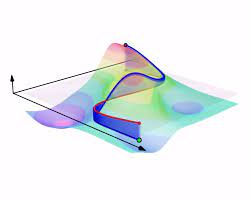
\includegraphics[scale=1.2]{figuras/imagen}
\vfill
BRYAN RICARDO BARBOSA OLVERA \\
\today \\

\end{center}
\end{titlepage}


\LARGE
\raggedleft
\color{blue}
\raggedright
\color{black}
Profesor: Jorge G. Macias Díaz \\
Edificio: 117 \\
Oficina: 6:30 - 3:30 \\
Email: Jemacias@correo.uaa.mx \\
Email Secundario: jorge.maciasdiaz@edu.uaa.mx \\
Tel: +4494527006 \\
\section{INTEGRALES DOBLES} 

\color{red} 
$\mathbf{Def.}$
\color{black} 
Un rectangulo en $\mathbb{R} ^2$ es 
$$ R = \left[ a_1,b_1  \right]  \times \left[ a_2 , b_2 \right] \subseteq \mathbb{R}^2 $$
Definimos $ A \left( R \right) =  $ $"$Area de $R "$ = $ \left( b_1 -a_1 \right) \left( b_2-a_2 \right)  $ 
\centering
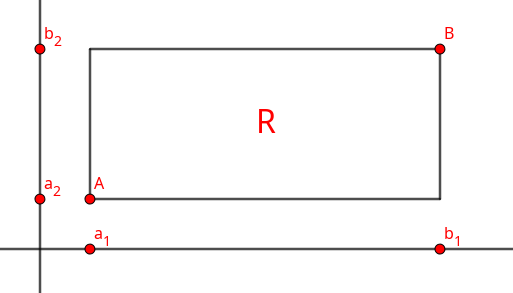
\includegraphics[scale=0.5]{figuras/img1 } \\
\raggedright
Sean 
$$\bar{a} = \left( a_1 , a_2 \right) $$
$$ \bar{b} = \left( b_1 , b_2 \right)  $$
\color{red}
Importante:
\color{black}
Haaser usa la notacion $ R = \left[ \bar{a} , \bar{b} \right]  $ \\
\color{red}
Obs.
\color{black}
Si $\mathcal{R} = \{ R \subseteq \mathbb{R} ^2 ; R$ es rectángulo  $\}$ ent \\
$ \mathcal{A}: \mathcal{R} \rightarrow \mathbb{R} ^+ \cup \{ 0 \} $ es una funcion. \\

\color{red} 
$\mathbf{Def.}$
\color{black} 
Sea $R= \left[ a_1 , b_1 \right] \times \left[ a_2,b_2 \right] \subseteq \mathbb{R}^2 $ una particion de $R$ es  
$$ \mathcal{P} = \mathcal{P}_1 \times \mathcal{P}_2 \ \text{con} $$
$ \mathcal{P}  $ es particicon de $[a_1,b_1]$ \\
$ \mathcal{P}  $ es particicon de $[a_2,b_2]$ \\
\newpage
Concretamente, Si 
$$ \mathcal{P}_1: a_1=x_0 < x_1 < \cdots < x_m = b_1 $$
$$ \mathcal{P}_2: a_2=y_0 < y_1 < \cdots < y_n = b_2$$
$$ \mathcal{P}= \{ \left( x_i , y_j \right) \in \mathbb{R} ^2 \textbar i=0,1,\cdots ,m ; j=0,1,\cdots ,n  \} $$
\centering

\includegraphics[scale=0.7]{figuras/img2 } \\
\raggedright
Definimos  
$R_{ij} = \left[ x_{i-1} , x_i \right] \times [y_{j-1}, y_j] \ \forall \ i=1,\cdots ,m \ \forall \ j=1, \cdots, n  $  \\ 
\color{red} Obs. \color{black} $ R = \cup_{i=1}^{m} \cup_{j=1}^{n}R_{ij} $ \\
\color{red} 
$\mathbf{Def.}$
\color{black} 
Definimos la norma de $\mathcal{P}$ como 
$$ \abs{  \mathcal{P} } = \text{max} \{ \abs{ \mathcal{P}_1 , \mathcal{P}_2 } \} $$
$$ \abs{\mathcal{P}_1} = \text{max} \{ x_i -x_{i-1} \textbar i=1,\cdots, m  \} $$
$$ \abs{\mathcal{P}_2} = \text{max} \{ y_j -y_{j-1} \textbar j=1,\cdots, n  \} $$
\color{red} Obs \color{black} Con la notacion de la definicion anterior 
$$ \mathcal{A} \left( R \right) = \sum_{i=1}^{m} \sum_{j=1}^{n} \mathcal{A} \left( R_{ij} \right)  $$
\color{red} Dem. \color{black} \\
$$ 
\sum_{i=1}^{m} \sum_{j=1}^{n} \left( \mathcal{A} \left( R_{ij} \right) \right) = 
\sum_{i=1}^{m} \sum_{j=1}^{n} \left( x_i - x_{i-1} \right) \left( y_j - y_{j-1} \right) =
$$
$$
= \sum_{i=1}^{m} \left( x_i-x_{i-1} \right)   \sum_{j=1}^{n}  \left( y_j - y_{j-1} \right) = 
\sum_{i=1}^{m} \left( x_i-x_{i-1} \right)  \left( b_2 -a_2 \right)  = 
$$
$$
= \left( b_2-a_2 \right)   \sum_{i=1}^{m} \left( x_i-x_{i-1} \right)  = 
 \left( b_2-a_2 \right)  \left( b_1-a_1 \right) =
 \mathcal{A} \left( R \right)  \ 
$$
\begin{flushright}
$\blacksquare$
\end{flushright}

\color{red} 
$\mathbf{Def.}$
\color{black} 
Definimos 
$$ \wp \left( R \right) = \{ \mathcal{P} \textbar \mathcal{P} \text{ particion de  } R \}  $$

\color{red} 
$\mathbf{Def.}$
\color{black} 
Sea  $R$ un rectangulo $R = \left[ a_1,b_1 \right] \times [a_2,b_2] \subseteq \mathbb{R} ^2$. \\
Sean $\mathcal{P} , \mathcal{P}^{\prime} \subset \wp \left( R \right)  $ \\
Diga  
$$ \mathcal{P} = \mathcal{P}_1 \times \mathcal{P}_2 \wedge  \mathcal{P}^{\prime} = \mathcal{P}_1^{\prime} \times 
\mathcal{P}_2^{\prime} $$
decimos $\mathcal{P}^{\prime}$ es refinamiento de $\mathcal{P}$ \\
Si $\mathcal{P}_1 \subseteq \mathcal{P}_1^{\prime} \wedge \mathcal{P}_2 \subseteq \mathcal{P}_2^{\prime}$ \\
Notacion: $\mathcal{P} \subseteq \mathcal{P}^{\prime}$ \\
\color{red} Obs. \color{black} En lo que sigue: 
$$ R = \left[ a_1, b_1 \right] \times \left[ a_2, b_2 \right]  \subseteq \mathbb{R}^2 \wedge f: R \rightarrow 
\mathbb{R} \ \ \  \text{es acotada} $$
Mas aún, $m,M \in \mathbb{R} \ni $ 
$$ \forall \ x \in \mathbb{R} \ : m \leq f \left( x \right) \leq M $$

\color{red} 
$\mathbf{Def.}$
\color{black} 
Sea $\mathcal{P} = \mathcal{P_1} \times \mathcal{P_2} \in \wp \left( \mathbb{R} \right)  $ \\
Diga 
$$\mathcal{P}_1: a_1 =x_0 <x_1< \cdots < x_m = b_1  $$
$$\mathcal{P}_2: a_2 =y_0 <y_1< \cdots < y_m = b_2  $$
Definimos 
$$ L \left( f, \mathcal{P} \right) = "\text{Suma inferior de $f$ con respecto a } \mathcal{P} " $$
$$ = \sum_{i=1}^{m} \sum_{j=1}^{n} m_{ij} \left( f \right) \mathcal{A} \left( R_{ij} \right)  $$
con $ m_{ij} \left( f \right) = \text{inf} \{ f \left( x \right) \textbar x \in R_{ij} \}   $ 
\newpage
Definimos 
$$ U \left( f, \mathcal{P} \right) = "\text{Suma superior de $f$ con respecto a } \mathcal{P} " $$
$$ = \sum_{i=1}^{m} \sum_{j=1}^{n} M_{ij} \left( f \right) \mathcal{A} \left( R_{ij} \right)  $$
con $ M_{ij} \left( f \right) = \text{sup} \{ f \left( x \right) \textbar x \in R_{ij} \}   $ \\
\color{red} 
$\mathbf{Lemma.}$
\color{black} 
 $\forall \ \mathcal{P} \in \wp \left( R \right) : $
 $$ m \mathcal{A} \left( R \right) \leq L \left( f,\mathcal{P} \right) \leq U \left( f, \mathcal{P} \right) \leq M \mathcal{A}$$
\color{red} 
$\mathbf{Dem.}$ \\
\color{black} 
$$ m \mathcal{A} \left( R \right) = 
m \sum_{i=1}^{m} \sum_{j=1}^{n} \mathcal{A} \left( R_{ij} \right) =    
 \sum_{i=1}^{m} \sum_{j=1}^{n} m \mathcal{A} \left( R_{ij} \right)     
$$
$$
\leq 
 \sum_{i=1}^{m} \sum_{j=1}^{n} m_{ij} \left( f \right) \mathcal{A} \left( R_{ij} \right)
= L \left( f,\mathcal{P} \right) $$
$$
\leq \sum_{i=1}^{m} \sum_{j=1}^{n} M_{ij} \left( f \right) \mathcal{A} \left( R_{ij} \right) 
= U \left( f, \mathcal{P} \right) 
$$
$$
\leq
\sum_{i=1}^{m} \sum_{j=1}^{n} M  \mathcal{A} \left( R_{ij} \right)  = 
M \sum_{i=1}^{m} \sum_{j=1}^{n}  \mathcal{A} \left( R_{ij} \right) = 
M \mathcal{A} \left( R \right) 
$$
$$ \therefore
m \mathcal{A} \left( R \right) \leq L \left( f ,\mathcal{P} \right) \leq 
U \left( f,\mathcal{P} \right)  \leq M \mathcal{A} \left( R \right) 
$$
\begin{flushright}
$\blacksquare$
\end{flushright}
\color{red} 
$\mathbf{Def.}$
\color{black} 
Definimos 
$$ \mathscr{L} \left( f \right) = " \text{Conjunto de sumas superiores de  } f "  $$
$$ = \{ L \left( f, \mathcal{P} \right) \textbar \mathcal{P} \in \wp \left( R \right)   \}  $$
$$ \mathscr{U} \left( f \right) = " \text{Conjunto de sumas inferiores de  } f "  $$
$$ = \{ U \left( f, \mathcal{P} \right) \textbar \mathcal{P} \in \wp \left( R \right)   \}  $$
\newpage
\color{red} 
$\mathbf{Obs.}$
\color{black} 
Del lema anterior. 
$$ \forall L \left( f,\mathcal{P} \right) \in \mathscr{L} \left( f \right) : L \left( f , \mathcal{P} \right) \subseteq
 M \mathcal{A} \left( R \right)  $$
Asi, $ \emptyset \neq \mathscr{L} \left( f \right)  $ acotado sumeriormente 
$\Rightarrow \ \exists \ \text{sup } \mathscr{L} \left( f \right) $ \\
Similarmente $\exists \ \text{inf} \mathscr{U} \left( f \right)  $ \\
\color{red} 
$\mathbf{Def.}$
\color{black} 
Definimos 
\begin{gather*}
    \upint_R f = "\text{Integral inferior de } f \text{ sobre } R "= \text{ sup } \mathscr{L} \left( f \right)    \\
    \lowint_R f = "\text{Integral superior de } f \text{ sobre } R "= \text{ inf } \mathscr{U} \left( f \right)    \\ 
\end{gather*}

\color{red} 
$\mathbf{Lemma}$
\color{black} 
Sean $\mathcal{P} , \mathcal{P} ^{\prime} \in \wp \left( R \right) \ni \mathcal{P} \subseteq \mathcal{P} ^{\prime} $. Entonces
$$ m \mathcal{A} \left( R \right) \leq L \left( f ,\mathcal{P} \right) \leq L \left( f , \mathcal{P} ^{\prime} \right) 
\leq  U \left( f,\mathcal{P}^{\prime}  \right) \leq U \left( f , \mathcal{P} \right) \leq M \mathcal{A} \left( R \right)    $$
\color{red} 
$\mathbf{Dem.}$ \\
\color{black} 
Sean \\
$$\mathcal{P} = \mathcal{P}_1 \times \mathcal{P}_2 \in \wp \left( R \right)  $$
$$\mathcal{P}^{\prime} = \mathcal{P}_1^{\prime} \times \mathcal{P}_2^{\prime} \in \wp \left( R \right)  $$
\color{red} 
$\mathbf{Caso1.}$
\color{black} 
$\mathcal{P}_1 = \mathcal{P}_1^{\prime}$. Sea  \\ 
$n = $ card $ \{ \mathcal{P}_2^{\prime} \backslash  \mathcal{P}_2  \} \ \in \ \mathbb{N} \cup \ \{ 0 \} $
Usaremos inducción sobre  $n$ \\
Si $n=0$, Ent. $\mathcal{P}_2 ^{\prime}= \mathcal{P}_2 $ \\ 
$ \mathcal{P} ^{\prime} = \mathcal{P} $, Ent. 
$$ L \left( f, \mathcal{P} \right) = L \left( f, \mathcal{P} ^{\prime} \right) \leq  U \left( f, \mathcal{P}^{\prime}  \right) 
= U \left( f, \mathcal{P}  \right) $$
\color{red} 
$\mathbf{Paso General:}$
\color{black} 
Supongamos la conclusion valida para algun $n \in \mathbb{N} \cup \{0 \} $ \\ 
veremos que es valido para $n+1$. Sea $ \mathcal{P}_2 ^{\prime}  $ refinamiento de $\mathcal{P}_2 \ \ni$  \\
$ n+1 = \text{ card } \left( \mathcal{P}_2 ^{\prime} \backslash  \mathcal{P}_2  \right)   $ \\
\newpage
Definimos $\mathcal{P}_2 \subseteq \mathcal{P}_2^{\prime \prime} \subseteq \mathcal{P}_2^{\prime} $
con  \\
card $ \left( \mathcal{P}_2 ^{ \prime \prime }  \backslash \mathcal{P}_2  \right) = n \ \wedge $ 
card $ \left( \mathcal{P}_2 ^{ \prime  }  \backslash \mathcal{P}_2^{\prime \prime}  \right) = 1  $ \\
por hipótesis  de inducción:
$$ L \left( f, \mathcal{P}  \right) \leq L \left( f, \mathcal{P} ^{\prime \prime}   \right) \leq 
U \left( f, \mathcal{P}^{\prime \prime}  \right) \leq U \left( f , \mathcal{P}  \right)   $$
donde $ \mathcal{P}^{\prime \prime} = \mathcal{P}_2  \times  \mathcal{P}_2^{\prime \prime}   $ \\ 
Digo 
$$ \mathcal{P}_2^{\prime \prime} : a_2 = y_0 <y_1< \cdots < y_{j_0} < y_{j_{0+1}} < \cdots < y_p = b_2 $$
$$ \mathcal{P}_2^{\prime } : a_2 = y_0 <y_1< \cdots < y_{j_0}<y^{*} < y_{j_{0+1}} < \cdots < y_p = b_2 $$
$$ \mathcal{P}_1 : a_1 = x_0 <x_1 < x_m = b_1 $$
\color{red} 
$\mathbf{Obs.}$
\color{black} 
$$ L \left( f, \mathcal{P}  \right) = \sum_{i=1}^{m} \sum_{j=1}^{p} 
\left( \text{inf} _{ \left[ x_{i-1} , x_i \right] \times \left[ y_{j-1}, y_j \right]   } \right) \cdot  \mathcal{A} 
 \left( \left[ x_{i-1}, x_i \right] \times \left[ y_{j-1} , y_j \right]   \right)   $$
$$
= \sum_{i=1}^{m}  \sum_{{j=1,j\neq j_0 +1} } ^{p} \left( \text{inf} _ { \left[ x_{i-1}, x_i \right] \times \left[ y_{j-1}, y_j \right]  } \right)  
\cdot \mathcal{A} \left( \left[ x_{i-1} , x_i \right] \times \left[ y_{j-1},y_j \right]   \right)  
$$
$$
+  \sum_{i=1}^{m} \left( \text{inf}_{ \left[ x_{i-1},x_i \right] \times \left[ y_{j_0} , y_{j_0 +1} \right]   } \right)  \cdot 
\mathcal{A} \left( \left[ x_{i-1} , x_i \right] \times \left[ y_{j_0} , y_{j_0 +1} \right]   \right)   
$$

$$
= \sum_{i=1}^{m}  \sum_{{j=1,j\neq j_0 +1} } ^{p} \left( \text{inf} _ { \left[ x_{i-1}, x_i \right] \times \left[ y_{j-1}, y_j \right]  } \right)  
\cdot \mathcal{A} \left( \left[ x_{i-1} , x_i \right] \times \left[ y_{j-1},y_j \right]   \right)  
$$
$$
+  \sum_{i=1}^{m} \left( \text{inf}_{ \left[ x_{i-1},x_i \right] \times \left[ y_{j_0} , y^{*} \right]   } \right)  \cdot 
\mathcal{A} \left( \left[ x_{i-1} , x_i \right] \times \left[ y_{j_0} , y^{*} \right]   \right)   
$$ 
$$ + \sum_{i=1}^{m} \left( \text{inf}_{ \left[ x_{i-1},x_i \right] \times \left[ y^{*} , y_{j_0+1} \right]   } \right)  \cdot 
\mathcal{A} \left( \left[ x_{i-1} , x_i \right] \times \left[ y^{*} , y_{j_0 +1} \right]   \right)   
$$
$$ = L \left( f , \mathcal{P}^{\prime}  \right) \leq U \left( f, \mathcal{P} ^{\prime}  \right) \leq U \left( f, \mathcal{P} ^{\prime}  \right) \leq U \left( f , \mathcal{P} ^{ \prime \prime }  \right)     $$
(El caso 1 se sigue por inducción) 

\color{red} 
$\mathbf{Caso 2:}$
\color{black} 
$ \mathcal{P}_2  = \mathcal{P}_2 ^{\prime} \ \wedge \ \mathcal{P}_1 \subseteq \mathcal{P} _1 ^{\prime}  $ similar al caso 1

\newpage
\color{red} 
$\mathbf{Caso3:}$
\color{black} 
$ \mathcal{P}_1 \subseteq \mathcal{P}_1 ^{\prime} \ \wedge \ \mathcal{P}_2 \subseteq \mathcal{P}_2 ^{\prime} $ \\
$$ \mathcal{P} = \mathcal{P}_1 \times \mathcal{P}_2    $$
$$ \mathcal{P} ^{\prime} = \mathcal{P}_1 \times \mathcal{P}_2^{\prime}    $$
Definimos $\mathcal{P} ^{\prime \prime} = \mathcal{P}_1 \times \mathcal{P}_2 ^{\prime}   $ de los casos anteriores
$$ L \left( f , \mathcal{P} \right) \leq L \left( f, \mathcal{P} ^{\prime \prime}  \right) \leq 
U \left( f, \mathcal{P }^{\prime}  \right) \leq U \left( f, \mathcal{P}^{\prime \prime}  \right) \leq 
U \left( f, \mathcal{P}  \right)  $$
\begin{flushright}
$\blacksquare$
\end{flushright}

\color{blue}
\begin{flushright}
9/8/2023
\end{flushright}
\color{black}
\color{red} 
$\mathbf{Lemma}$
\color{black} 
Sea $R \subseteq R^2$ rectángulo, $f : R \rightarrow \mathbb{R} $ acotada y $m,M \ \in \ \mathbb{R} \ \ni$ 


\end{document}
